\documentclass{beamer}
\usepackage{multicol}
\usepackage{graphicx}
\usepackage{tikz}
\usepackage{tikzscale}
\usepackage[english]{babel}
\usepackage{amsmath}
\usepackage{amssymb}
\usepackage{mathtools}
\usepackage{mathrsfs}
\usepackage{xcolor}
\usepackage{physics}
\usepackage{bm}
\usepackage{bbm}
\usetheme[alternativetitlepage=bild]{Rub}
\renewcommand{\vec}[1]{\bm{#1}}
\begin{document}
\title{Gaussian Random Field Generation \\for stochastic PDEs}   
\author{Timo Schorlepp} 
\date{\today} 
\titlegraphic{titel.png}
\frame{\titlepage} 

\frame{\frametitle{Table of contents}\tableofcontents} 

%%%%%%%%%%%%%%%%%%%%%%%%%%%%%%%%%%%%%%%%%%%%%%%%%
\section{Motivation} 
%%%%%%%%%%%%%%%%%%%%%%%%%%%%%%%%%%%%%%%%%%%%%%%%%
\frame{\frametitle{Motivation:\\Exemplary applications} 
\begin{columns}[t]
\column{.5\textwidth}
\centering
\includegraphics[width=.65\textwidth]{figures/cosmogrf}\\
\tiny{
Vogelsberger et al. 2014, Illustris simulation}\\
\includegraphics[width=.65\textwidth]{figures/2dns}\\
\tiny{Murray 2017, 2$D$ stochastic NSE vorticity}
\column{.5\textwidth}
\centering
\includegraphics[width=.65\textwidth]{figures/kpz}\\
\tiny{Kuennen, Wang 2008, KPZ surface growth}\\[.2cm]
\includegraphics[width=.65\textwidth]{figures/aquifer}\\
\tiny{Wikimedia, aquifer sketch}
\end{columns}
}
%%%%%%%%%%%%%%%%%%%%%%%%%%%%%%%%%%%%%%%%%%%%%%%%%
\frame{\frametitle{Motivation:\\Mathematical examples} 
Deterministic incompressible NSE for $\vec{u}:\mathbb{T}^d \times \mathbb{R}_+ \to \mathbb{R}^d$:
\begin{align*}
\partial_t \vec{u} + (\vec{u} \cdot \nabla) \vec{u} + \nabla p = \nu \Delta \vec{u}\; , \; \nabla \cdot \vec{u} = 0 
\end{align*}
Without forcing: 
\begin{align*}
\dv{}{t} \int \mathrm{d}V \; \frac{1}{2} \abs{\vec{u}}^2 = - 2 \nu \int \mathrm{d}V \; \trace((\nabla \otimes \vec{u})^T (\nabla \otimes \vec{u})) \leq -2 C \nu \int \mathrm{d}V \; \abs{\vec{u}}^2
\end{align*}
Gronwall: Energy decays exponentially, need forcing for interesting long-term behavior, e.g. Gaussian forcing with homogeneous, isotropic correlation matrix!\\
\medskip
Similarly: Stochastic heat equation\\
Why Gaussian? CLT, easy, algorithms exist
}
%%%%%%%%%%%%%%%%%%%%%%%%%%%%%%%%%%%%%%%%%%%%%%%%%
\section{Theory} 
%%%%%%%%%%%%%%%%%%%%%%%%%%%%%%%%%%%%%%%%%%%%%%%%%
\subsection{Basic Definitions}
%%%%%%%%%%%%%%%%%%%%%%%%%%%%%%%%%%%%%%%%%%%%%%%%%
\frame{\frametitle{Theory:\\Basic Definitions}
\begin{block}{Definition 1}
A random field $\vec{\xi}$ is an indexed family of random variables
\begin{align*}
\vec{\xi} = \left\{ \vec{\xi}(\vec{x}) : \Omega \to \mathbb{R}^m \; ; \; \vec{x} \in T \subseteq \mathbb{R}^d \right\}.
\end{align*}
\end{block}
\begin{alertblock}{Remark 2}
\begin{itemize}
\item Generalization of stochastic processes
\item No details on Kolmogorov Existence Theorem etc. here
\end{itemize}
\end{alertblock}
}
%%%%%%%%%%%%%%%%%%%%%%%%%%%%%%%%%%%%%%%%%%%%%%%%%
\frame{\frametitle{Theory:\\Basic Definitions}
\begin{block}{Definition 3}
A random field $\vec{\xi}$ is called Gaussian iff $\forall k \in \mathbb{N}: \forall \{\vec{x}^{(0)}, \cdots , \vec{x}^{(k-1)} \} \subseteq T: \vec{\xi}(\vec{x}^{(0)}) =: \vec{\xi}^{(0)}, \cdots \vec{\xi}(\vec{x}^{(k-1)})=: \vec{\xi}^{(k-1)}$ are jointly normally distributed, i.e.
\begin{align*}
p_{\vec{\xi}^{(0)}, \cdots ,\vec{\xi}^{(k-1)}}(\vec{y}^{(0)}, \cdots \vec{y}^{(k-1)}) = &\det(2 \pi \Sigma)^{- \frac{1}{2}} \cdot \\ & \cdot \exp(-\frac{1}{2} (\vec{y}-\vec{\mu})^T \Sigma^{-1} (\vec{y}-\vec{\mu}))
\end{align*}
where $\Sigma$ is the $km \times km$ covariance matrix 
\begin{align*}
\Sigma_{m r + i,m s + j} = \text{Cov}\left(\xi^{(r)}_i,\xi^{(s)}_j \right) =: \chi_{ij}\left(\vec{x}^{(r)}, \vec{x}^{(s)} \right)
\end{align*}
and $\vec{\mu}$ is the $km$-dim.\ mean vector $\mu_{mr + i} = \left< \xi^{(r)}_i \right>$.
\end{block}
}
%%%%%%%%%%%%%%%%%%%%%%%%%%%%%%%%%%%%%%%%%%%%%%%%%
\frame{\frametitle{Theory:\\Basic Definitions}
\begin{alertblock}{Remark 4}
\begin{itemize}
\item Gaussian random fields (GRF) are completely specified by $\vec{\mu}(\vec{x})$ and $\chi \left(\vec{x}',\vec{x}\right)$ $\Longrightarrow$ easy!
\item We will assume $\vec{\mu}(\vec{x}) \equiv 0$ wlog in the following (also necessary for isotropy) as well as $d=m$
\item $\Sigma$ needs to be positive semidefinite for all $\vec{x}^{(0)},\cdots, \vec{x}^{(k-1)}$ since $\sum_{i,j}\vec{a}_i^T \chi \left(\vec{x}^{(i)},\vec{x}^{(j)}\right) \vec{a}_j = \text{Var}\left(\sum_{i} \vec{a}_i^T \vec{\xi}^{(i)} \right)\geq 0$\\
\end{itemize}
\end{alertblock}
}
%%%%%%%%%%%%%%%%%%%%%%%%%%%%%%%%%%%%%%%%%%%%%%%%%
\frame{\frametitle{Theory:\\Basic Definitions}
\begin{exampleblock}{Example/Definition 5}
\begin{itemize}
\item White noise $\chi_{ij}\left(\vec{x}',\vec{x}\right) = \delta(\vec{x}'-\vec{x}) \delta_{ij}$
\item Homogeneous (translation-invariant, stationary), isotropic ($O(n)$-invariant) and solenoidal correlation tensor:
\begin{align*}
\chi_{ij}(\vec{x}', \vec{x}) = \chi_{ij}(\vec{x}'-\vec{x}) = \chi_{ij}(\vec{r}) = f(r) \delta_{ij} + \frac{r f'(r)}{d-1} \left( \delta_{ij}-\frac{r_i r_j}{r^2}\right)
\end{align*}
\item Stationary diagonal correlation $\chi_{ij}(\vec{x}',\vec{x}) = \chi_0 \exp(-\frac{\abs{\vec{x}'-\vec{x}}}{\lambda}) \delta_{ij}$
\end{itemize}
\end{exampleblock}
\begin{alertblock}{Remark 6}
We do not distinguish between correlation and covariance matrices here (they differ by a constant factor in the stationary case)
\end{alertblock}
}
%%%%%%%%%%%%%%%%%%%%%%%%%%%%%%%%%%%%%%%%%%%%%%%%%
\subsection{How to generate stationary GRFs}
%%%%%%%%%%%%%%%%%%%%%%%%%%%%%%%%%%%%%%%%%%%%%%%%%
\frame{\frametitle{Theory:\\How to generate stationary GRFs}
\begin{exampleblock}{Example 7}
Assuming we can generate independent $\mathcal{N}(0,1)$ samples, how do we generate vectors $\vec{\xi} \sim \mathcal{N}(0,C)$ for a given covariance $d \times d$-matrix $C$?\\
\medskip
Answer: $C$ is positive semidefinite, allowing for a Cholesky or eigenvalue/-vectors decomposition $C=B^T B$, so if we sample $\vec{\phi}$ with independent $\mathcal{N}(0,1)$ entries, we get
\begin{align*}
\left< B^T \vec{\phi} \;  (B^T \vec{\phi})^T \right> = B^T \underbrace{\left< \vec{\phi} \vec{\phi}^T \right>}_{=I_d} B = B^T B = C
\end{align*}
\end{exampleblock}
}
%%%%%%%%%%%%%%%%%%%%%%%%%%%%%%%%%%%%%%%%%%%%%%%%%
\frame{\frametitle{Theory:\\How to generate stationary GRFs}
\begin{block}{Theorem 8 (Direct method)}
Let 
\begin{align*}
G = \left\{ \left( j_1 \frac{L_1}{N_1} , \cdots , j_d \frac{L_d}{N_d} \right) \; ; j_s \in \{ 0 , 1 , 2 , \cdots , N_s - 1   \} \right\}
\end{align*}
be a uniformly spaced grid in $[0,L_1] \times \cdots \times [0,L_d]$. Decomposing the overall $(N_1 \cdots N_d d) \times (N_1 \cdots N_d d)$ grid covariance matrix $\Sigma = \Lambda^T \Lambda$ of the grid and sampling $\vec{\phi} \sim \mathcal{N}(0,I_{N_1 \cdots N_d d})$ yields
\begin{align*}
\Lambda^T \vec{\phi} \sim \mathcal{N}(0,\chi)
\end{align*}
\end{block}
\begin{alertblock}{Remark 9}
Decomposing this matrix becomes prohibitively expensive really fast!
\end{alertblock}
}
%%%%%%%%%%%%%%%%%%%%%%%%%%%%%%%%%%%%%%%%%%%%%%%%%
\frame{\frametitle{Theory:\\How to generate stationary GRFs}
\begin{exampleblock}{Example 10}
Grid covariance matrix for stationary $\chi$ on $2D$ $8 \times 8$ grid:
\centering
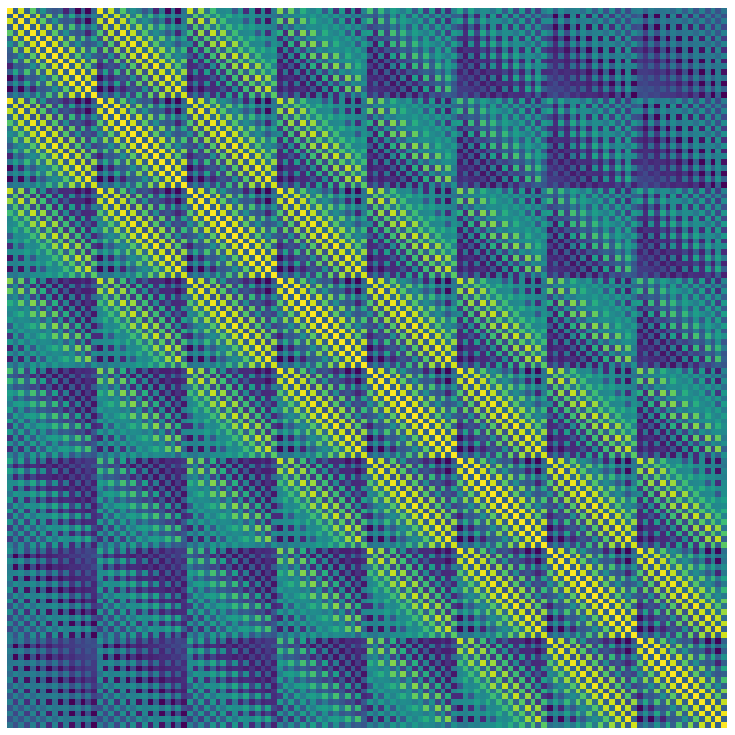
\includegraphics[width=.45\textwidth]{figures/bttb}\\
Block Toeplitz matrix (BTM)
\end{exampleblock}
}
%%%%%%%%%%%%%%%%%%%%%%%%%%%%%%%%%%%%%%%%%%%%%%%%%
\frame{\frametitle{Theory:\\How to generate stationary GRFs}
\begin{exampleblock}{Example 10 (continued, circulant embedding)}
Idea: Embed the BTM into a block \textit{circulant} matrix (BCM) by extending the grid with periodic boundary conditions. Goal: Use properties of BCMs (eigenvalues may be found via FFT of the individual $d \times d$ blocks)\\
\centerline{
\includegraphics[width=0.44\textwidth]{figures/embedgrd}
}
\end{exampleblock}
}
%%%%%%%%%%%%%%%%%%%%%%%%%%%%%%%%%%%%%%%%%%%%%%%%%
\frame{\frametitle{Theory:\\How to generate stationary GRFs}
\begin{alertblock}{Remark 10 (circulant embedding)}
\begin{itemize}
\item The extended covariance matrix need not be positive (semi)definite!\\
$\Longrightarrow$ Grid may need to be very large  
\item No further details here, check the literature list on last slide if you are interested in circulant embedding methods
\end{itemize}
\end{alertblock}
}
%%%%%%%%%%%%%%%%%%%%%%%%%%%%%%%%%%%%%%%%%%%%%%%%%
\section{Numerical implementation}
%%%%%%%%%%%%%%%%%%%%%%%%%%%%%%%%%%%%%%%%%%%%%%%%%
\frame{\frametitle{Title}
.
}


\section{Results} 
\frame{\frametitle{Title}
.
}


\section{Conclusion}
\frame{\frametitle{Title}

\begin{block}{A}
bla
\end{block}

\begin{exampleblock}{B}
bla
\end{exampleblock}


\begin{alertblock}{C}
bla
\end{alertblock}
}

\section{Literature}
\frame{\frametitle{Literature:\\Recommendations for further reading}
\begin{itemize}
\item A.\ Yaglom, Correlation Theory of Stationary and Related Random Functions, Springer Series in Statistics, 1987.
\item P.\ Abrahamsen, A Review of Gaussian Random Fields and Correlation Functions, Norsk Regnesentral/Norwegian Computing Center, 1997.
\item G.\ Chan, A.\ T.\ A.\ Wood, Simulation of stationary Gaussian vector fields, Statistics and Computing, 1999.
\item A. Lang, J. Potthoff, Fast simulation of Gaussian random fields, Monte Carlo Methods and Applications, 2011.

\end{itemize}
}

\end{document}
 